\documentclass[12pt]{article}
\usepackage[onehalfspacing]{setspace}
\usepackage{dcolumn}
\usepackage[left=1in, top=1in, bottom=1in]{geometry}
\usepackage{graphicx}
\usepackage[table,xcdraw]{xcolor}
\usepackage{longtable}
\usepackage{float}
\usepackage{listings}
\usepackage{xcolor}
\usepackage{amsmath}
\usepackage{amsfonts}
\usepackage{amssymb}


\lstset{language=R,
    basicstyle=\small\ttfamily,
    stringstyle=\color{commentgreen},
    otherkeywords={0,1,2,3,4,5,6,7,8,9},
    morekeywords={TRUE,FALSE},
    deletekeywords={data,frame,length,as,character},
    keywordstyle=\color{blue},
    commentstyle=\color{commentgreen},
}
\begin{document}

\title{Syndicate 5 Statistical Learning Problem Set \#3}
\maketitle
{\setlength{\parindent}{0cm}


\section*{CD4 percentage level in child with HIV}
\subsection*{Question 1}
The model allowing for random effects on the intercept across different child patients can be modelled as:

$$CD4PCT_i = \alpha_{j[i]} + \beta time_i + \epsilon_i$$
$$\alpha_j = \mu_\alpha + \eta_j$$
$$\eta_j \sim N(0, \sigma^2_\alpha)$$

Using the lme4 package to get estimates for our parameters we obtain the model below:

$$CD4PCT_i = \alpha_{j[i]} -3.3001 time_i + \epsilon_i$$
$$\alpha_j = 25.4729 + \eta_j$$
$$\eta_j \sim N(0, \sigma^2_\alpha)$$


\subsection*{Question 2}
The model allowing for treatment and the child's age at their initial visit to explain the random intercept can be modelled as:

$$CD4PCT_i = \alpha_{j[i]} + \beta time_i + \epsilon_i$$
$$\alpha_j = \gamma_0 + \gamma_1 treatment_j + \gamma_2 baseage_j + \eta_j$$
$$\eta_j \sim N(0, \sigma^2_\alpha)$$

Using the lme4 package to get estimates for our parameters we obtain the model below:

$$CD4PCT_i = \alpha_{j[i]} -3.2686 time_i + \epsilon_i$$
$$\alpha_j = 27.6231 + 1.9074 treatment_j -0.9259 baseage_j + \eta_j$$
$$\eta_j \sim N(0, \sigma^2_\alpha)$$

Looking at the output, time still has a negative impact on CD4 percentages in a child's blood. However, treatment has a positive impact on the child specific intercept while a child's base age has has a negative impact on on the child specific intercept. In other words, while a child's CD4 percentage levels decrease over time, their initial levels are higher if the child had undertaken the new treatment course yet lower for groups (individual children) who started the treatment at older ages. Notably, while $time_i$ and $baseage_j$ are significant at the 1\% level, $treatment_j$ isn't even significant at the 10\% level so it likely has little effect on a child's base CD4 levels.\\

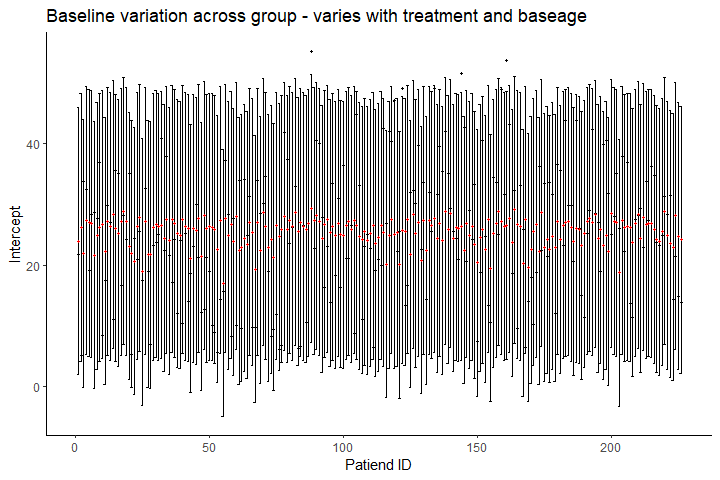
\includegraphics[scale=0.6]{Q2}

Plotting the child specific intercepts, we can see that the mean intercept for each child now changes depending on if they've undergone treatment and what their age was at the start of the treatment.

MENTION SOMETHING ABOUT VARIATION COMPARED TO IDIOSYNCRATIC VARIATION


\subsection*{Question 3}
The multiple linear model can be modelled as below:
$$CD4PCT_i = \beta_0 + \beta_1 time_i + \beta_2 treatment_j + \beta_3 baseage_j + \epsilon_i$$
Using OLS we get the estimates below:
$$CD4PCT_i = 27.2739 -2.2862 time_i + 2.7089 treatment_j -0.9158 baseage_j + \epsilon_i$$












\begin{table}[!htbp] \centering 
  \caption{} 
  \label{} 
\begin{tabular}{@{\extracolsep{5pt}}lccc} 
\\[-1.8ex]\hline 
\hline \\[-1.8ex] 
 & \multicolumn{3}{c}{\textit{Dependent variable:}} \\ 
\cline{2-4} 
\\[-1.8ex] & \multicolumn{3}{c}{CD4PCT} \\ 
\\[-1.8ex] & \multicolumn{2}{c}{\textit{linear}} & \textit{OLS} \\ 
 & \multicolumn{2}{c}{\textit{mixed-effects}} & \textit{} \\ 
\\[-1.8ex] & (1) & (2) & (3)\\ 
\hline \\[-1.8ex] 
 time & $-$3.300$^{***}$ & $-$3.269$^{***}$ & $-$2.286$^{***}$ \\ 
  & (0.518) & (0.518) & (0.881) \\ 
  & & & \\ 
 treatment &  & 1.907 & 2.709$^{***}$ \\ 
  &  & (1.588) & (0.842) \\ 
  & & & \\ 
 baseage &  & $-$0.926$^{***}$ & $-$0.916$^{***}$ \\ 
  &  & (0.351) & (0.188) \\ 
  & & & \\ 
 Constant & 25.473$^{***}$ & 27.623$^{***}$ & 27.274$^{***}$ \\ 
  & (0.845) & (1.598) & (0.992) \\ 
  & & & \\ 
\hline \\[-1.8ex] 
Observations & 978 & 978 & 978 \\ 
R$^{2}$ &  &  & 0.041 \\ 
Adjusted R$^{2}$ &  &  & 0.038 \\ 
Log Likelihood & $-$3,572.420 & $-$3,567.026 &  \\ 
Akaike Inf. Crit. & 7,152.839 & 7,146.052 &  \\ 
Bayesian Inf. Crit. & 7,172.381 & 7,175.365 &  \\ 
Residual Std. Error &  &  & 13.102 (df = 974) \\ 
F Statistic &  &  & 14.004$^{***}$ (df = 3; 974) \\ 
\hline 
\hline \\[-1.8ex] 
\textit{Note:}  & \multicolumn{3}{r}{$^{*}$p$<$0.1; $^{**}$p$<$0.05; $^{***}$p$<$0.01} \\ 
\end{tabular} 
\end{table} 





























}
\end{document}